\documentclass[]{book}
\usepackage{lmodern}
\usepackage{amssymb,amsmath}
\usepackage{ifxetex,ifluatex}
\usepackage{fixltx2e} % provides \textsubscript
\ifnum 0\ifxetex 1\fi\ifluatex 1\fi=0 % if pdftex
  \usepackage[T1]{fontenc}
  \usepackage[utf8]{inputenc}
\else % if luatex or xelatex
  \ifxetex
    \usepackage{mathspec}
  \else
    \usepackage{fontspec}
  \fi
  \defaultfontfeatures{Ligatures=TeX,Scale=MatchLowercase}
\fi
% use upquote if available, for straight quotes in verbatim environments
\IfFileExists{upquote.sty}{\usepackage{upquote}}{}
% use microtype if available
\IfFileExists{microtype.sty}{%
\usepackage{microtype}
\UseMicrotypeSet[protrusion]{basicmath} % disable protrusion for tt fonts
}{}
\usepackage[margin=1in]{geometry}
\usepackage{hyperref}
\hypersetup{unicode=true,
            pdftitle={Podstawy programowania R},
            pdfauthor={Łukasz Wawrowski},
            pdfborder={0 0 0},
            breaklinks=true}
\urlstyle{same}  % don't use monospace font for urls
\usepackage{natbib}
\bibliographystyle{plainnat}
\usepackage{longtable,booktabs}
\usepackage{graphicx,grffile}
\makeatletter
\def\maxwidth{\ifdim\Gin@nat@width>\linewidth\linewidth\else\Gin@nat@width\fi}
\def\maxheight{\ifdim\Gin@nat@height>\textheight\textheight\else\Gin@nat@height\fi}
\makeatother
% Scale images if necessary, so that they will not overflow the page
% margins by default, and it is still possible to overwrite the defaults
% using explicit options in \includegraphics[width, height, ...]{}
\setkeys{Gin}{width=\maxwidth,height=\maxheight,keepaspectratio}
\IfFileExists{parskip.sty}{%
\usepackage{parskip}
}{% else
\setlength{\parindent}{0pt}
\setlength{\parskip}{6pt plus 2pt minus 1pt}
}
\setlength{\emergencystretch}{3em}  % prevent overfull lines
\providecommand{\tightlist}{%
  \setlength{\itemsep}{0pt}\setlength{\parskip}{0pt}}
\setcounter{secnumdepth}{5}
% Redefines (sub)paragraphs to behave more like sections
\ifx\paragraph\undefined\else
\let\oldparagraph\paragraph
\renewcommand{\paragraph}[1]{\oldparagraph{#1}\mbox{}}
\fi
\ifx\subparagraph\undefined\else
\let\oldsubparagraph\subparagraph
\renewcommand{\subparagraph}[1]{\oldsubparagraph{#1}\mbox{}}
\fi

%%% Use protect on footnotes to avoid problems with footnotes in titles
\let\rmarkdownfootnote\footnote%
\def\footnote{\protect\rmarkdownfootnote}

%%% Change title format to be more compact
\usepackage{titling}

% Create subtitle command for use in maketitle
\newcommand{\subtitle}[1]{
  \posttitle{
    \begin{center}\large#1\end{center}
    }
}

\setlength{\droptitle}{-2em}
  \title{Podstawy programowania R}
  \pretitle{\vspace{\droptitle}\centering\huge}
  \posttitle{\par}
  \author{Łukasz Wawrowski}
  \preauthor{\centering\large\emph}
  \postauthor{\par}
  \date{}
  \predate{}\postdate{}

\usepackage{booktabs}
\usepackage{amsthm}
\makeatletter
\def\thm@space@setup{%
  \thm@preskip=8pt plus 2pt minus 4pt
  \thm@postskip=\thm@preskip
}
\makeatother

\begin{document}
\maketitle

{
\setcounter{tocdepth}{1}
\tableofcontents
}
\chapter*{Wprowadzenie}\label{wprowadzenie}
\addcontentsline{toc}{chapter}{Wprowadzenie}

Literatura podstawowa:

\begin{itemize}
\tightlist
\item
  Przemysław Biecek -
  \href{http://pbiecek.github.io/Przewodnik/}{\emph{Przewodnik po
  pakiecie R}}
\item
  Marek Gągolewski -
  \href{http://www.gagolewski.com/publications/programowanier/}{\emph{Programowanie
  w języku R. Analiza danych, obliczenia, symulacje.}}
\item
  Garret Grolemund, Hadley Wickham -
  \href{http://r4ds.had.co.nz/}{\emph{R for Data Science}}
\end{itemize}

Literatura dodatkowa:

\begin{itemize}
\tightlist
\item
  \href{https://github.com/mi2-warsaw/SER/blob/master/histoRia/README.md}{inne
  pozycje po polsku}
\item
  \href{https://bookdown.org/}{inne pozycje po angielsku}
\end{itemize}

\chapter{Wprowadzenie do R}\label{wprowadzenie-do-r}

GNU R to interpretowany język programowania oraz środowisko do obliczeń
statystycznych i wizualizacji wyników {[}Wikipedia 2017{]}.

Robert A. Muenchen - \href{http://r4stats.com/articles/popularity/}{The
Popularity of Data Science Software}

\begin{figure}
\centering
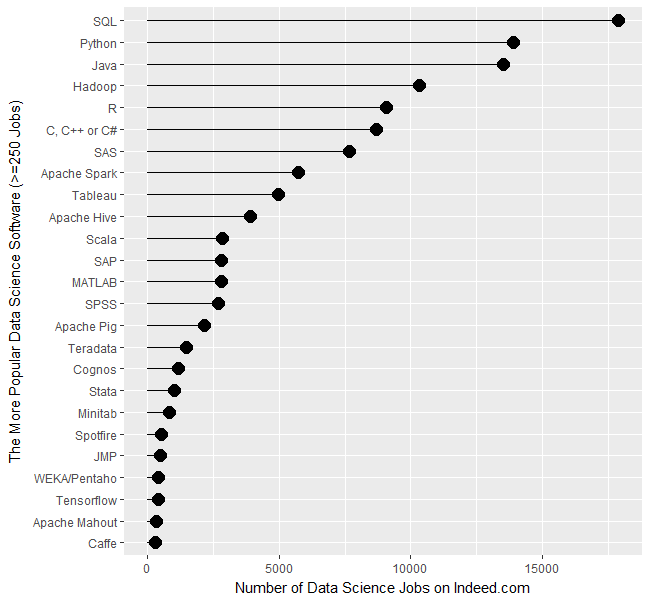
\includegraphics{img/pop_r1.png}
\caption{}
\end{figure}

\section{R}\label{r}

Bazowa wersja R jest do pobrania ze strony
\href{https://cloud.r-project.org/}{r-project.org}.

\begin{figure}
\centering
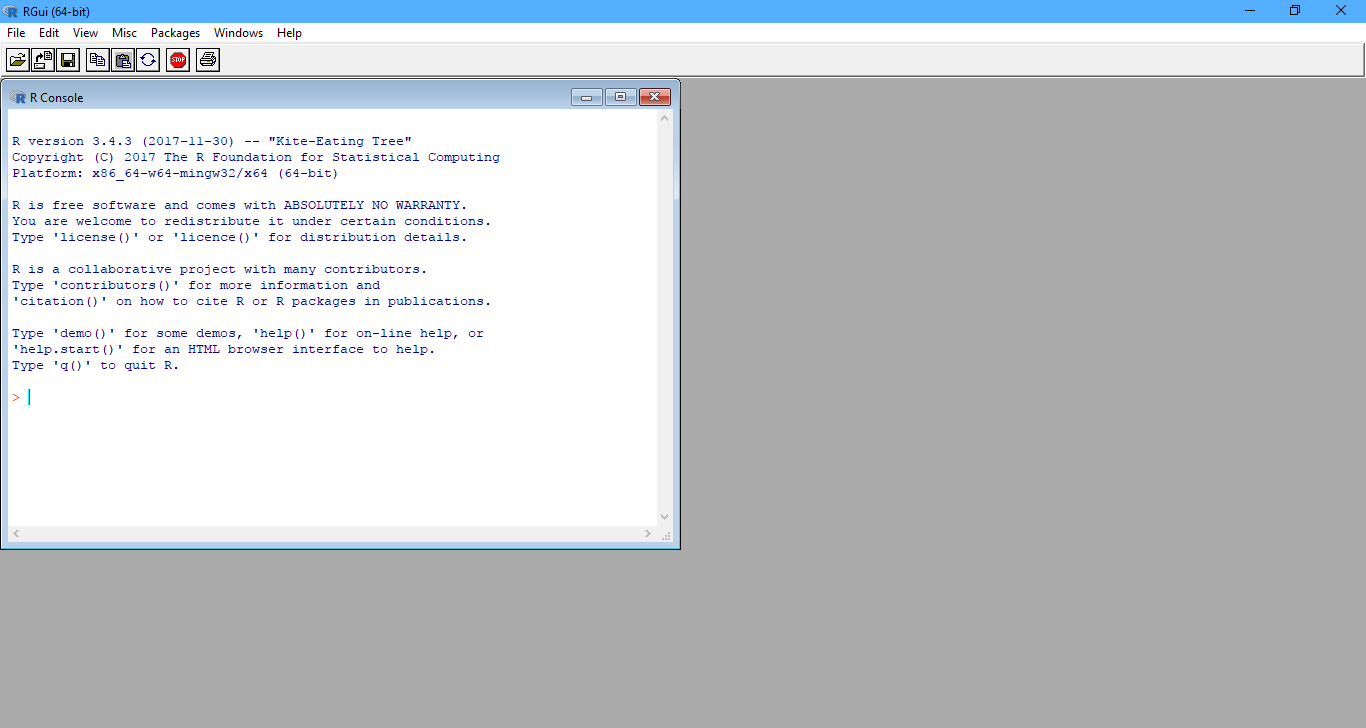
\includegraphics{img/r.png}
\caption{}
\end{figure}

\section{RStudio}\label{rstudio}

RStudio to zintegrowane środowisko programistyczne (IDE) dla języka R
dostępne za darmo na stronie
\href{https://www.rstudio.com/products/rstudio/download/}{RStudio}.

\begin{figure}
\centering
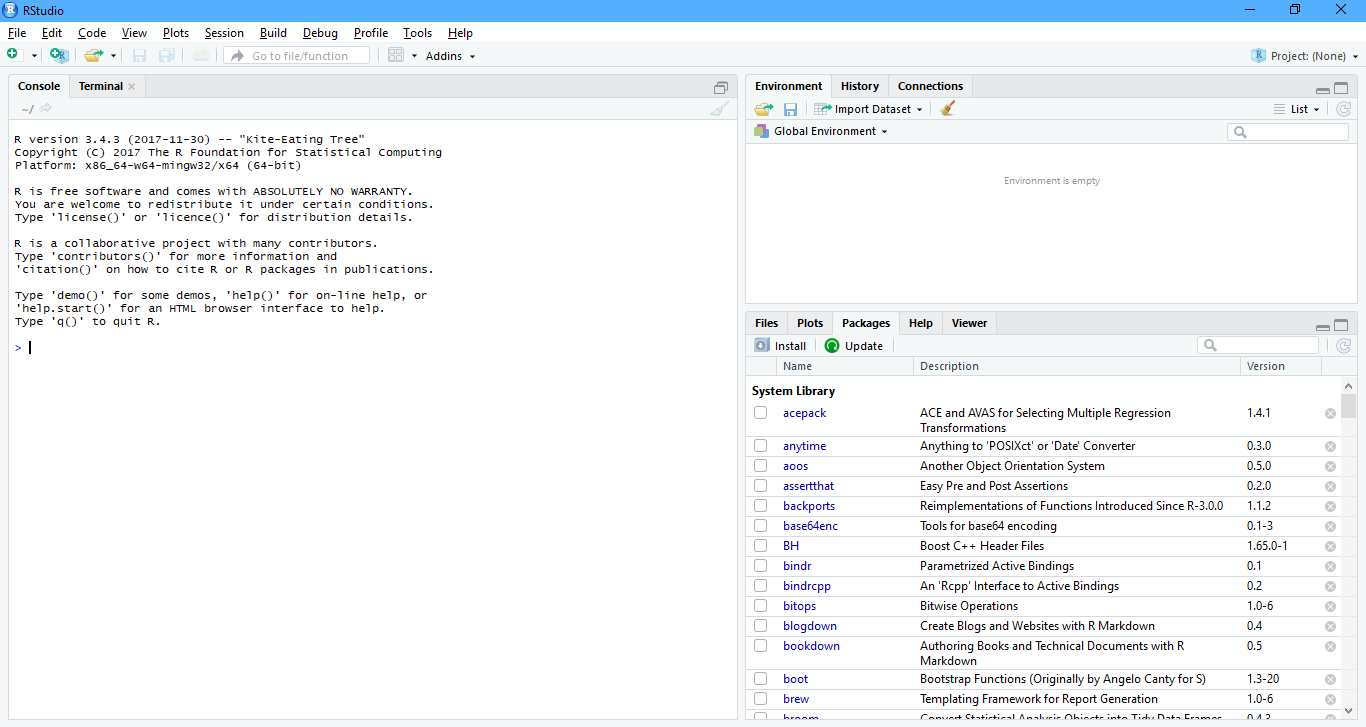
\includegraphics{img/rstudio.png}
\caption{}
\end{figure}

Z R można także korzystać w
\href{https://www.visualstudio.com/pl/vs/rtvs/}{Microsoft Visual
Studio}.

\textbf{W codziennej pracy RStudio jest wygodniejsze, jednak długotrwałe
obliczenia lepiej uruchamiać w zwykłym R.}

\section{Pakiety}\label{pakiety}

Podstawowe możliwości R są dosyć ograniczone. Rozszerzają je pakiety,
których obecnie jest ponad 12 tysięcy. Można je przeglądać według
kategorii w \href{https://cran.r-project.org/web/views/}{CRAN Task
Views} lub w wygodnej wyszukiwarce
\href{https://www.r-pkg.org/}{METACRAN}.

\chapter{Struktury danych}\label{struktury-danych}

\section{Wektor}\label{wektor}

\section{Macierz}\label{macierz}

\section{Faktor/czynnik}\label{faktorczynnik}

\section{Lista}\label{lista}

\section{Ramka danych}\label{ramka-danych}

\section{Braki danych}\label{braki-danych}

\section{Import danych}\label{import-danych}

\chapter{Przetwarzanie danych}\label{przetwarzanie-danych}

\section{Pakiet tidyverse}\label{pakiet-tidyverse}

\section{Wybieranie kolumn}\label{wybieranie-kolumn}

\section{Filtrowanie}\label{filtrowanie}

\section{Dodawanie nowych zmiennych}\label{dodawanie-nowych-zmiennych}

\section{Grupowanie}\label{grupowanie}

\section{Podsumowanie}\label{podsumowanie}

\section{Łączenie zbiorów}\label{aczenie-zbiorow}

\section{Wąska i szeroka reprezentacja
danych}\label{waska-i-szeroka-reprezentacja-danych}

\chapter{Programowanie w R}\label{programowanie-w-r}

\section{Funkcje}\label{funkcje}

\section{Pętle}\label{petle}

\section{Instrukcje warunkowe}\label{instrukcje-warunkowe}

\chapter{Wizualizacja danych}\label{wizualizacja-danych}

\section{Wbudowane funkcje}\label{wbudowane-funkcje}

\section{Pakiet ggplot2}\label{pakiet-ggplot2}


\end{document}
